\section{Data model}
\FloatBarrier
\begin{figure}[ht]
	\centering
	\centerline{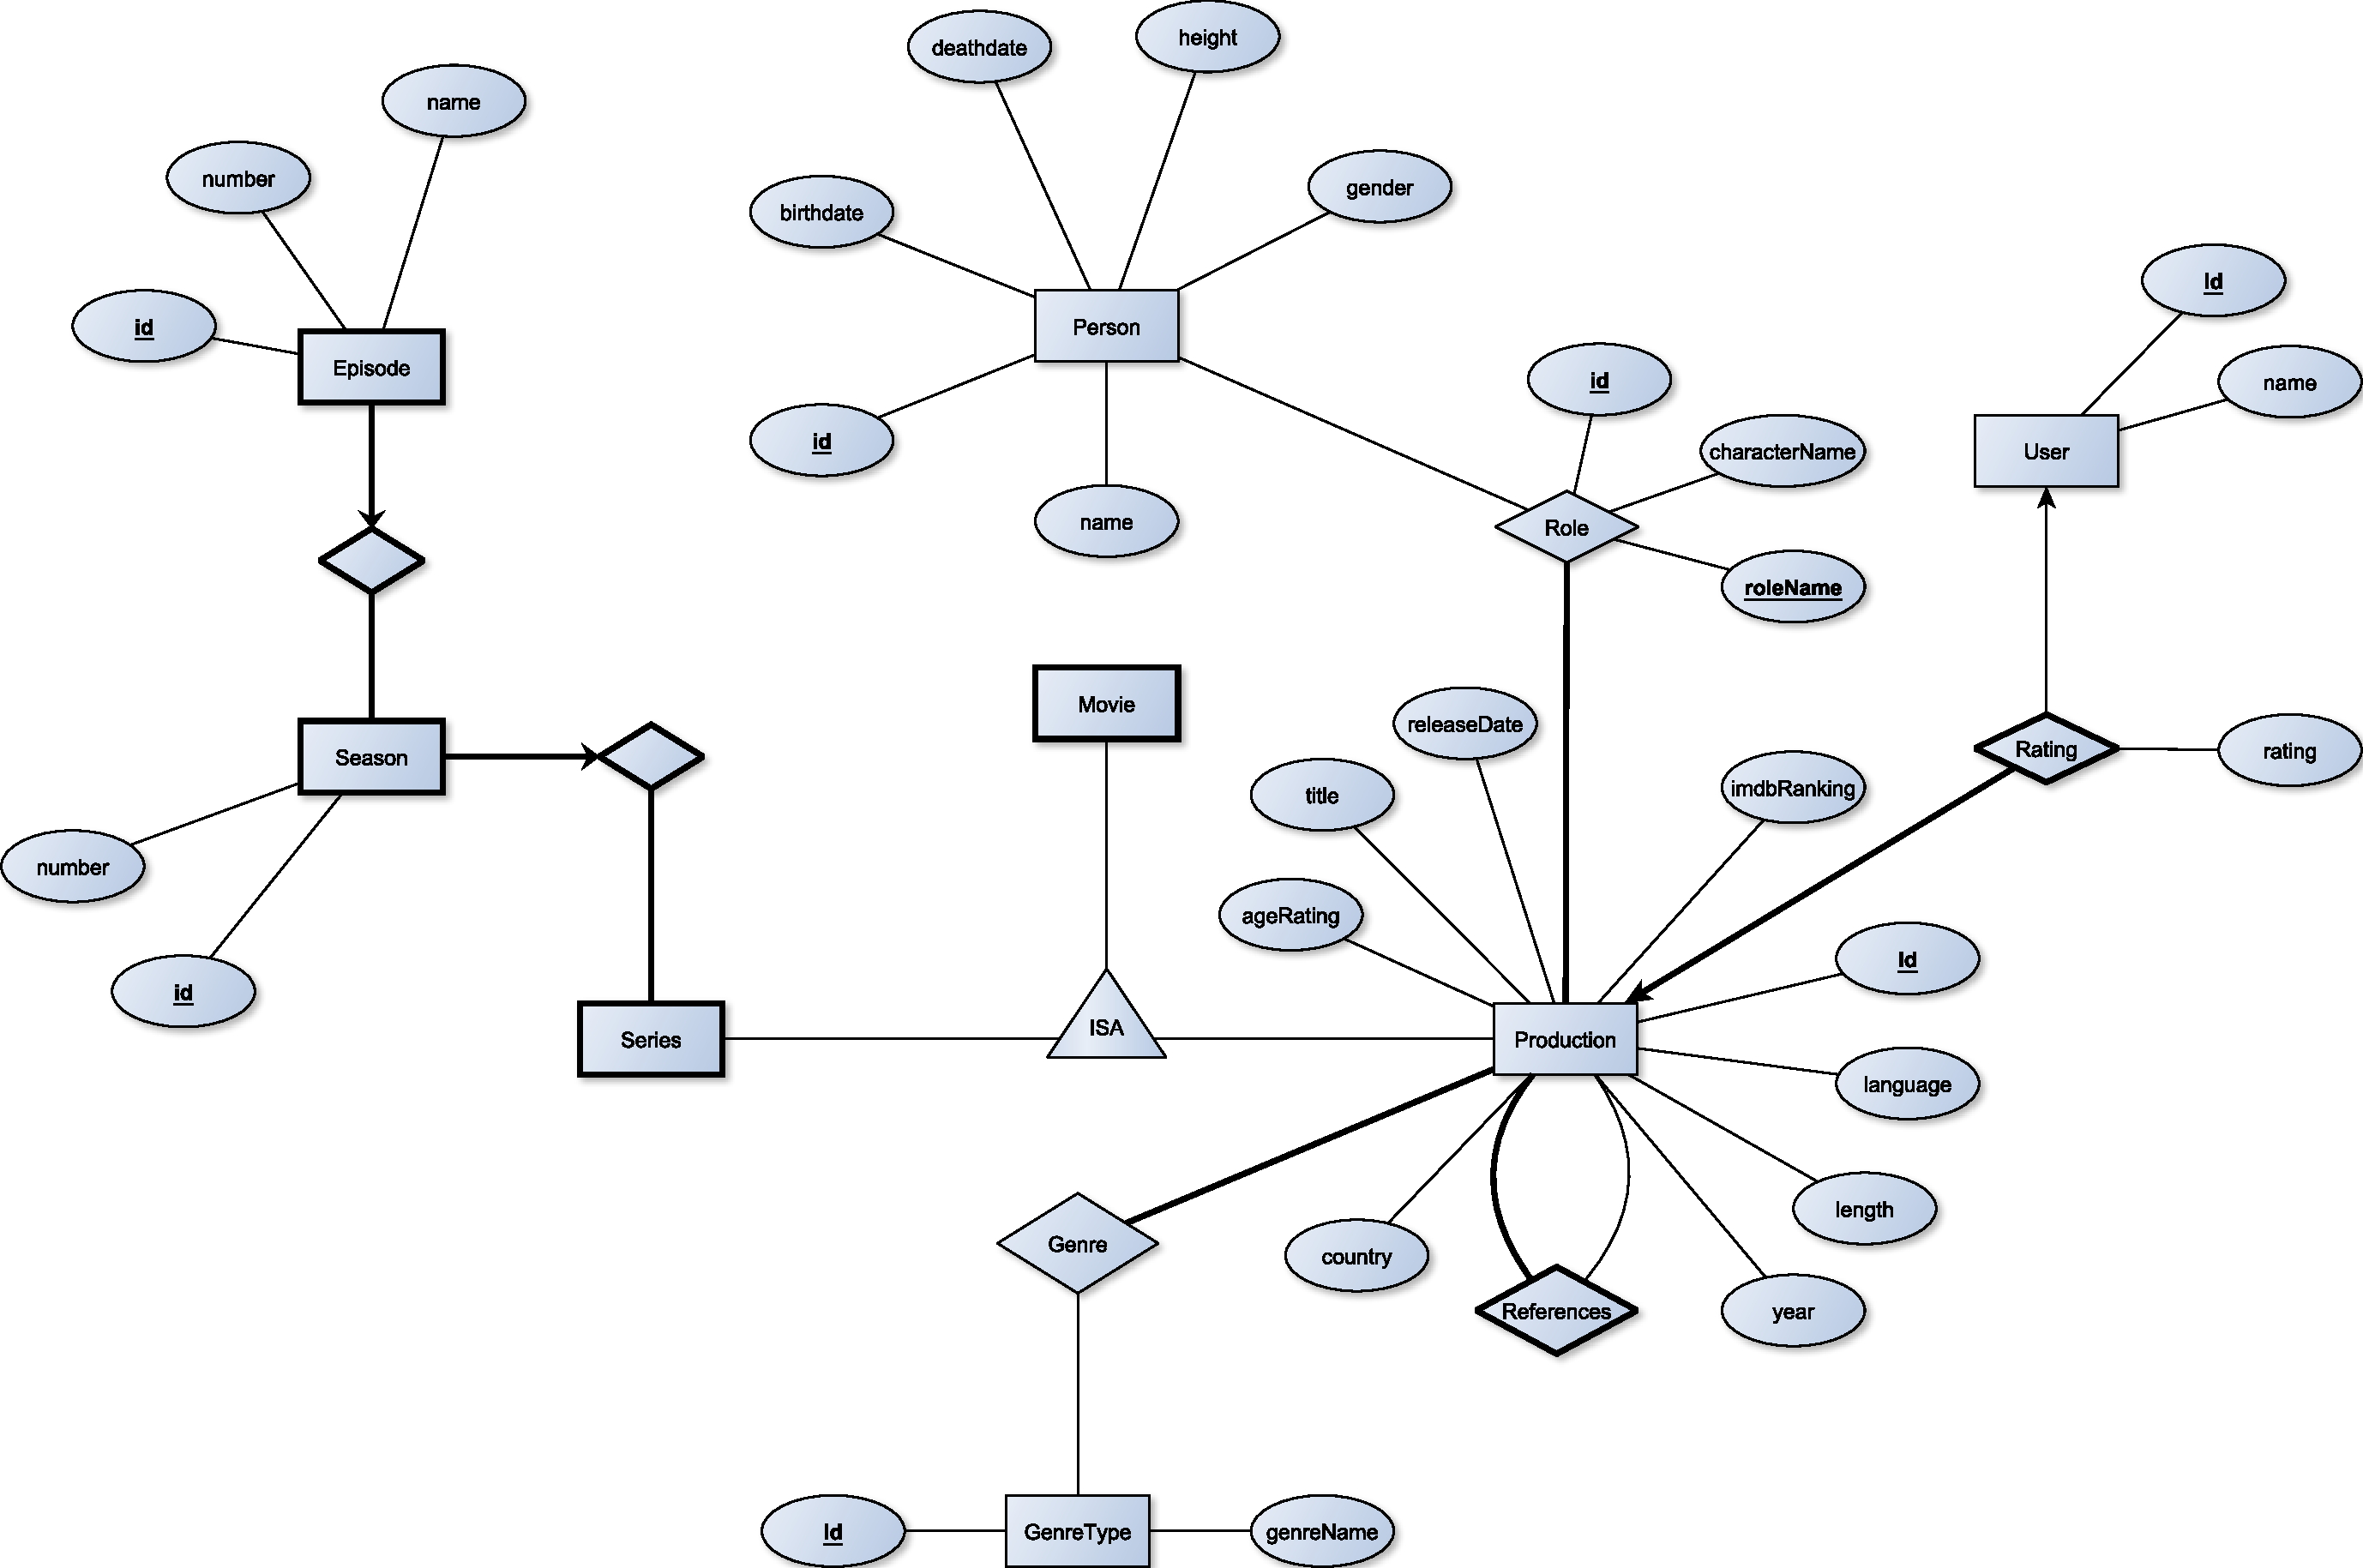
\includegraphics[scale=0.35]{figures/ERD.pdf}}
	\caption{Entity-relationship model}
\end{figure}
\FloatBarrier

\subsection{Revision}
\subsubsection{Removed contract}
The Contract relation was removed, as it was realized that this relation provided only redundant information, as it simply referenced from one relation to its relationship-table with another relation, thus becoming an unnecessary obstacle when it comes to retrieving data regarding and/or requiring the connection between the Person and Production relations. Thus "Role" is now the only connecting relation between these two aforementioned relations. Role now acts as the sole relationship-table between them, as well as defining what role the person has in regards to the production. A person can thereby be both an actor and a director for a production, and because the Role table contains a "characterName" value, this table can also represent several acting roles of a person in a single production.

\subsubsection{Removed IDs from Series and Season}
Since a series and a season are productions themselves, they need not have an ID defined for themselves.

\subsubsection{ISA > Relationship-notation}
We swapped the relationship notation going from Production to Series and Movie with an ISA notation, to further define that a series or movie is indeed a production.

\subsubsection{Added Reference relation}
As we lacked the information from the IMDB database defining which movies refer to other movies, we added this relation to our own database, to be able to represent exactly this information.

\subsubsection{Added users and their ratings of productions}
To be able to solve the SQL-query assignments discussing the votes of students for various movies in the IMDB database, we realized we had to represent this information as well. We decided to store these students' ratings in the Rating relation, connecting this to the User relation, which then stores information about the users themselves.

\subsubsection{Updated notation-form}
We removed all number-indications of whether a connection between two relations is many-to-many, one-to-one, etc. as the lines between the various relations and their relationships should be read as the notifying factor for this information.